\begin{figure}[ht]\centering
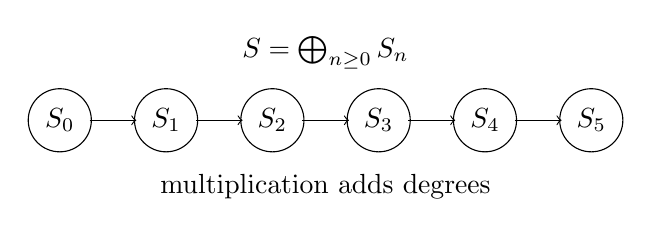
\begin{tikzpicture}[x=1.35cm,y=.8cm]
\foreach \n in {0,...,5}{\node[draw,circle,minimum size=8mm] at (\n,0) {\(S_{\n}\)};}
\foreach \n in {0,...,4}{\draw[->] (\n+.28,0)--(\n+.72,0);}
\node[above] at (2.5,.65) {\(S=\bigoplus_{n\ge0}S_n\)};
\node[below] at (2.5,-.7) {multiplication adds degrees};
\end{tikzpicture}
\caption{The grading decomposes the ring into degree pieces.}\label{fig:vi34-02}\end{figure}